\documentclass[12pt]{article}
\usepackage{graphicx} % Required for inserting images
\usepackage{natbib}
%\usepackage{fullpage}
\usepackage[dvipsnames]{xcolor}
\usepackage[%
plainpages,%
colorlinks,% removes the boxes around links
urlcolor=black,%
filecolor=black,%
linkcolor=Blue,
citecolor=Blue,%   requires xcolor with option dvipsnames
pdfpagemode=UseOutlines,%
pdfauthor={Lars Vilhuber},%
pdfsubject={Analysis Validation at Scale},%
]{hyperref}
\usepackage{acronym}
\usepackage{setspace}
%TCIDATA{Version=5.00.0.2570}
%TCIDATA{LaTeXparent=0,0,sw-edit.tex}

% $Id: acrodefs.tex 6859 2017-07-05 20:00:01Z lv39 $
% $URL: https://forge.cornell.edu/svn/repos/jma7/sloan-synthetic-data-server/text/acrodefs.tex $
%
% Define acronyms to be used in the text here. See
% http://www.mackichan.com/index.html?techtalk/456.htm~mainFrame for usage in
% Scientific workplace context


% head -11 $(find . -name acronyms.tex -exec ls -l --full-time {} \; | sort -k 6 | tail -1 | awk ' { print $9 } ')  > /ramdisk/acronyms.tex
%cat $(find . -name acronyms.tex -exec ls -l --full-time {} \; | sort -k 6 | awk ' { print $9 } ') | sort | uniq > /ramdisk/acronyms.tex

\acrodef{ACS}{American Community Survey}
\acrodef{ACS-POW}{American Community Survey Place of Work file}
\acrodef{ACS-PUMS}{American Community Survey Public Use Microdata Sample}
\acrodef{AEA}{American Economic Association}
\acrodef{AHEAD}{Study of Assets and Health Dynamics Amongst the Oldest Old}
\acrodef{AHS}{American Housing Survey}
\acrodef{ASCII}{American Standard Code for Information  Interchange} %, typically used to denote raw text files in PC or Unix environments
\acrodef{ASM}{Annual Survey of Manufacturers}
\acrodef{BB}{Bayesian bootstrap}
\acrodef{BCC}{Bowie Computer Center}
\acrodef{BDS}{Business Dynamics Statistics}
\acrodef{BED}{Business Employment Dynamics}
\acrodef{BES}{Business Expenditure Survey}
\acrodef{BIC}{Bayes Information Criterion}
\acrodef{BLS}{Bureau of Labor Statistics}
\acrodef{BMF}{Block Map File}
\acrodef{BRB}{Business Register Bridge}
\acrodef{BRB}{LEHD Business Register Bridge}
\acrodef{BR}{Business Register}
\acrodef{BR}{Business Register\acroextra{, formerly known as the SSEL}}
\acrodef{CAC}{Cornell Center for Advanced Computing}
\acrodef{CBO}{Congressional Budget Office}
\acrodef{CBP}{County Business Patterns}
\acrodef{CBSA}{Core Based Statistical Area}
\acrodef{CBSA}{Core-Based Statistical Area}
\acrodef{CER}{Covered Earnings Records}
\acrodef{CES}{Center for Economic Studies}
\acrodef{CEW}{Covered Employment and Wages}%. Employment statistics program run by BLS in  conjunction with all states, also known as ES-202. Generally, when used  in this document, refers to public-use tabulations from the CEW, as  opposed to the confidential microdata received directly from the states.
\acrodef{CFN}{Census File Number}
\acrodef{CIA}{Central Intelligence Agency}
\acrodef{CISER}{Cornell Institute for Social and Economic Research}
\acrodef{CIT}{Cornell Information Technologies}
\acrodef{CM}{Census of Manufactures}
\acrodef{CNSS}{Cornell National Social Survey}
\acrodef{CODA}{Children of the Depression Age}
\acrodef{Code1}{Code 1\acroextra{, geocoding software from Group 1, now owned by Pitney Bowes}}
\acrodef{COLA}{cost of living allowance}
\acrodef{CPI}{Consumer Price Index}
\acrodef{CPI-U}{Consumer Price Index (All Urban Consumers)}
\acrodef{CPR}{Composite Person Record}
\acrodef{CPS}{Current Population Survey}
\acrodef{CRADC}{Cornell Restricted Access Data Center}
\acrodef{CRDCN}{Canadian Research Data Center Network}
\acrodef{CRAN}{the Comprehensive R Archive Network\acroextra{, accessible at
\url{http://cran.r-project.org/} and natively within R}}
\acrodef{CSV}{Comma-separated values}
\acrodef{CTC}{Cornell Theory Center}
\acrodef{CTPP}{Census Transportation Planning Package}
\acrodef{DCC}{Data Confidentiality Committee}
\acrodef{DC}{Decennial Census}
\acrodef{DDI}{Data Documentation Initiative\acroextra{, see \href{http://www.ddialliance.org/}{http://www.ddialliance.org/}}}
\acrodef{err}{excess reallocation rate}
\acrodef{jcr}{job creation rate}
\acrodef{jdr}{job destruction rate}
\acrodef{jrr}{job reallocation rate}
\acrodef{wrr}{worker reallocation rate}
\acrodef{DER}{Detailed Earnings Record}
\acrodef{DHS}{Department of Homeland Security}
\acrodef{DMZ}{Demilitarized Zone}
\acrodef{DOI}{Digital Object Identifier}
\acrodef{DRB}{Disclosure Review Board}
\acrodef{DWS}{Displaced Worker Supplement}
\acrodef{ECF}{Employer Characteristics  File}
\acrodef{EHF}{Employment History Files}
\acrodef{EHRI}{Enterprise Human Resources Integration}
\acrodef{EIN}{\acroextra{(federal) }Employer Identification Number}
\acrodef{ERR}{Excess Reallocation Rate}
\acrodef{ES-202}{ES-202\acroextra{. An older name for the \ac{QCEW} program}}
\acrodef{FBI}{Federal Bureau of Investigation}
\acrodef{fCOI}{financial Conflict of Interest}
\acrodef{FDIC}{Federal Deposit Insurance Corporation}
\acrodef{FDZ}{Research Data Centre of the German Federal Employment Agency}
\acrodef{FEMA}{Federal Emergency Management Agency}
\acrodef{FHFA}{Federal Housing Finance Agency}
\acrodef{FIPS}{Federal information processing standards codes\acroextra{\ issued     by \ac{NIST}}}
\acrodef{FOIA}{Freedom of Information Act}
\acrodef{FSRDC}{Federal Statistical Research Data Center}
\acrodef{FTI}{Federal Tax Information}
\acrodef{FTI}{Federal Tax Information\acroextra{, typically covered under     Title 26, U.S.C.}}
\acrodef{GAL}{Geocoded Address List}
\acrodef{GAO}{Government Accountability Office}
\acrodef{GDPR}{General Data Protection Regulation}
\acrodef{GIS}{Geographic Information System}
\acrodef{GRF-C}{Geographic Reference File-Codes}
\acrodef{GRF}{Geographic Reference File}
\acrodef{GSA}{General Services Administration}
\acrodef{GSF}{Gold Standard File\acroextra{, for SIPP merged to administrative data}}
\acrodef{GSS}{General Social Survey}
\acrodef{HCEF}{100 Percent Census Edited File}
\acrodef{HDF}{100 Percent Detail File}
\acrodef{HHS}{\acroextra{Department of\ }Health and Human Services}
\acrodef{HIPAA}{Health Insurance Portability and Accountability Act}
\acrodef{HPI}{\ac{OFHEO} House Price Index}
\acrodef{HPC}{high performance computing}
\acrodef{HRS}{Health and Retirement Study}
\acrodef{ICF}{Individual Characteristics File}
\acrodef{ICPSR}{Inter-university Consortium for Political and Social Research}
\acrodef{IDC}{Iterative Database Construction}
\acrodef{IDSC}{International Data Service Center}
\acrodef{ILR}{Cornell School of Industrial and Labor Relations}
\acrodef{IPUMS}{Integrated Public Use Microdata Series}
\acrodef{IRB}{Institutional Review Board}
\acrodef{IRS}{Internal Revenue Service}
\acrodef{ISBN}{International Standard Book Number}
\acrodef{ISR}{Institute for Social Research}
\acrodef{ISSN}{International Standard Serial Number}
\acrodef{IZA}{Institute for the Study of Labor}
\acrodef{JCR}{Job Creation Rate}
\acrodef{JDR}{Job Destruction Rate}
\acrodef{JHF}{Job History File}
\acrodef{JOLTS}{Job Openings and Labor Turnover Survey}
\acrodef{JRR}{Job Reallocation Rate}
\acrodef{JSM}{Joint Statistical Meetings}
\acrodef{KDE}{kernel density estimator}
\acrodef{LAUS}{Local Area Unemployment Statistics}
\acrodef{LBDB}{\ac{LBD} Bridge}
\acrodef{LBD}{Longitudinal Business Database}
\acrodef{LDB}{\ac{BLS}'s Longitudinal Business Database}
\acrodef{LDI}{Labor Dynamics Institute\acroextra{, \url{http://www.ilr.cornell.edu/ldi/}}}
\acrodef{LED}{Local Employment Dynamics}
\acrodef{LEHD}{Longitudinal Employer-Household Dynamics}
\acrodef{LLM}{large language model}
\acrodef{LMI}{Labor Market Information}
\acrodef{LODES}{LEHD Origin-Destination Employment Statistics}
\acrodef{MAF}{Master Address File}
\acrodef{MBR}{Master Beneficiary Record}
\acrodef{MEF}{Master Earnings File}
\acrodef{MER}{Master Earnings Record}
\acrodef{MLS}{Mass Layoff Statistics}
\acrodef{MMS}{Methodology, Measurement, and Statistics}
\acrodef{MN}{Minnesota}
\acrodef{MOU}{Memorandum of Understanding}
\acrodef{MSA}{Metropolitan Statistical Area}
\acrodef{MSD}{Metropolitan Statistical Division}
\acrodef{MWR}{Multiple Worksite Report}
\acrodef{NAICS}{North American Industry Classification System}
\acrodef{NASEM}{National Academies of Science, Engineering, and Medecine}
\acrodef{NBER}{National Bureau of Economic Research}
\acrodef{NECTA}{New England  City and Town Area}
\acrodef{NIA}{National Institute on Aging}
\acrodef{NICF}{National \ac{ICF}}
\acrodef{NISS}{the National Institute of Statistical Sciences}
\acrodef{NIST}{National Institute of Standards and Technology}
\acrodef{NLSY79}{National Longitudinal Survey of Youth}
\acrodef{NLSY}{National Longitudinal Survey of Youth}
\acrodef{NORC}{NORC}
\acrodef{NQWI}{National \ac{QWI} }
\acrodef{NSF}{National Science Foundation}
\acrodef{NSTA}{NAICS SIC Treatment of Auxiliaries}
\acrodef{NYCRDC}{New York Census Research Data Center}
\acrodef{OFHEO}{Office of Federal Housing Enterprise Oversight\acroextra{, now part of \ac{FHFA} }}
\acrodef{OMB}{Office of Management and Budget}
\acrodef{OPM}{U.S. Office of Personnel Management}
\acrodef{OSP}{Office of Sponsored Programs}
\acrodef{OTM}{OnTheMap}
\acrodef{PCF}{Personal Characteristics File}
\acrodef{PCF}{Person Characteristics File}
\acrodef{PHF}{Person History File}
\acrodef{PIK}{Protected Identity Key}
\acrodef{PI}{Principal Investigator}
\acrodef{PNG}{Portable Network Graphics}
\acrodef{POI}{Point of information\acroextra{file, one of the OPM data files}}
\acrodef{PPC}{Post Project Certification}
\acrodef{PPD}{posterior predictive distribution}
\acrodef{PPF}{production possibilities frontier}
\acrodef{PPN}{Permanent Plant Number}
\acrodef{PPS}{Predominant Purpose Statement}
\acrodef{PSID}{Panel Study of Income Dynamics}
\acrodef{PUF}{public use file}
\acrodef{PUMF}{public-use microdata file}
\acrodef{PMW}{Private Multiplicative Weights}
\acrodef{QA}{quality assurance}
\acrodef{QCEW}{Quarterly Census of Employment and Wages\acroextra{, managed by   the \acf{BLS}}}
\acrodef{QWIPU}{Public-Use \ac{QWI}}
\acrodef{QWI}{Quarterly Workforce Indicators}
\acrodef{RDA}{Restricted Data Application}
\acrodef{RDC}{Research Data Center}
\acrodef{RHLS}{Retirement History Longitudinal Survey}
\acrodef{RUN}{Reporting unit number}
\acrodef{SCEF}{Sample Census Edited File}
\acrodef{SCF}{Survey of Consumer Finances}
\acrodef{SCT}{Standard Code Table\acroextra{, one of the OPM data files}}
\acrodef{SDL}{statistical disclosure limitation}
\acrodef{SDS}{Synthetic Data Server\acroextra{, see \url{http://www.vrdc.cornell.edu/sds/}}}
\acrodef{SDMX}{Statistical Data and Metadata eXchange\acroextra{, see \href{http://sdmx.org/}{http://sdmx.org}}}
\acrodef{SEDF}{Sample Edited Detail File}
\acrodef{SEIN}{State employer identification number\acroextra{. It is     constructed from the state \ac{FIPS} code and the UI account     number. The BLS refers to the UI account number in combination with the     reporting unit number as SESA-ID}}
\acrodef{SEINUNIT}{SEIN reporting unit}
\acrodef{SEINUNIT}{SEIN unit number\acroextra{, a establishment identifier within LEHD, corresponding to the ``reporting unit'' on the \ac{QCEW}}}
\acrodef{SEPB}{Summary of Earnings and Projected Benefits} % confidential SSA                                 file
\acrodef{SESA-ID}{State Employment Security Agency ID\acroextra{. The UI     account number in combination with the Reporting Unit Number is treated   as a unique establishment identifier.}}
\acrodef{SESA}{State Employment Security Agency}
\acrodef{SJIAOS}{Statistical Journal of the IAOS}
\acrodef{SIC}{Standard Industry Classification}
\acrodef{SIPP}{Survey of Income and Program Participation}
\acrodef{SLID}{Survey of Labour and Income Dynamics}
\acrodef{SOLE}{Society of Labor Economists}
\acrodef{SPF}{Successor-Predecessor File}
\acrodef{SRMI}{Sequential Regression Multiple Imputation}
\acrodef{SSA}{Social Security Administration}
\acrodef{SSB}{SIPP Synthetic Beta\acroextra{, constructed from the \ac{SIPP} linked to
\ac{SSA}/\ac{IRS} Form W-2 records and \ac{SSA} records of retirement and disability benefit
receipt}}
\acrodef{SSC}{Statistical Software Components\acroextra{, at
\url{http://econpapers.repec.org/software/bocbocode/}, and accessible from within Stata}}
\acrodef{SSI}{Supplemental Security Income}
\acrodef{SSN}{Social Security Number}
\acrodef{SSR}{Supplemental Security Record}
\acrodef{SSS}{Special Sworn Status}
\acrodef{SynLBD}{Synthetic \ac{LBD}\acroextra{, a synthetic microdata file at the establishment level}}
\acrodef{U2W}{Unit-to-Worker Impute}
\acrodef{UCLA}{University of California Los Angeles}
\acrodef{UI}{Unemployment Insurance}
\acrodef{USC}{U.S. Code}
\acrodef{USPS}{United States Postal Service}
\acrodef{VPN}{Virtual Private Network}
\acrodef{WARN}{Worker Adjustment and Retraining Notification Act}
\acrodef{WB}{War Babies}
\acrodef{WIA}{Workforce Investment Act}
\acrodef{WIB}{Workforce Investment Board}
\acrodef{WRR}{Worker Reallocation Rate}
\acrodef{WTP}{willingness to pay}
\acrodef{WTS}{Windows Terminal Services}
\acrodef{XSEDE}{Extreme Science and Engineering Discovery Environment\acroextra{, \url{http://www.xsede.org}}}
\acrodef{XML}{Extensible Markup Language}
% tail -14 $(find . -name acronyms.tex -exec ls -l --full-time {} \; | sort -k 6 | tail -1 | awk ' { print $9 } ')  > /ramdisk/acronyms.tex

% Usage in the later text:
%  \ac{acronym}         Expand and identify the acronym the first time; use
%                       only the acronym thereafter
%  \acf{acronym}        Use the full name of the acronym.
%  \acs{acronym}        Use the acronym, even before the first corresponding
%                       \ac command
%  \acl{acronym}        Expand the acronym without using the acronym itself.

\onehalfspacing
\usepackage{enumitem}
\setlist{noitemsep}

\title{A method for analysis validation at scale}
\author{Lars Vilhuber}
\date{August 2024}



\begin{document}

\maketitle

%\begin{abstract}
%I describe past experience with the validation server process over 10 years and several hundred users, as a means to provide proxy access to confidential data. As a modern replacement, I propose the use of containers. The use of containers ensures reproducibility, reliable portability, and enables scalability. Infrastructure can be outsourced to commercial providers or users, at little to no cost to data providers. The only likely limitation to full automation is the absence of automated output vetting algorithms at statistical agencies.
%\end{abstract}

\vspace*{0.15in}
\hspace{10pt}
  \small	
  \textbf{\textit{Keywords: }} {synthetic data; verification server; confidential data; reproducibility; validation}
  
\section{Overview}
\label{sec:overview}

Researchers have, for the past 50 years, argued for greater access to the detailed but confidential data that statistical agencies collect and curate. From the 1965 proposal by the Social Science Research
Council for ``a federal data center, with public access for researchers'' \citep[pg. 219]{anderson_american_2015} to later calls for similar expanded access \citep[e.g.][]{card_expanding_2010}, these requests have been met by increasing options for providing such access \citep{united_nations_managing_2007,schouten_remote_2003,weinberg_access_2007,cole_handbook_2021}. Public use data is just one of those dissemination mechanisms, but even when data are publicly available, researchers have regularly obtained access to confidential data to assess and verify the accuracy and reliability of public use data relative to alternate sources of data \citep[to cite just a few, ][]{larrimore_consistent_2008,armour_using_2016,alexander_inaccurate_2010,abraham_exploring_2013,abraham_reconciling_2020}. A steadily increasing number of physical or virtual access portals to confidential US data (through the \ac{FSRDC} or virtual enclaves like those provided by the \ac{BLS} or the Economic Research Service of the USDA) provide researchers with access. Yet that access pales with the quantity of publications that use the public use data.\footnote{Public use data are available through many sources, but \ac{IPUMS} alone counts nearly 5,000 publications that use census, \ac{ACS}, and \ac{CPS} data in the past 5 years (as of 2024-08-14), which is almost surely an undercount of the overall usage. The Census Bureau's Center for Economic Studies' working paper series is the closest proxy for the number of publications that use data in the \ac{FSRDC}, as it includes papers by both staff and researchers (though it does not include papers that use other agencies' data exclusively). It lists 241 working papers over the same time period, from usage of all data sources available within the \ac{FSRDC}.} 

One approach to improving access to confidential data is by creating reasonable ``facsimiles'' of confidential data, or ``synthetic data.'' First proposed by \citet{rubin_discussion_1993}, various methods have been proposed since then \citep[see ][ for overviews]{VilhuberAbowdReiter-SJIAOS2016,raghunathan_synthetic_2021}. However, researchers, when faced with novel technology and datasets, are rightly suspicious of the data quality and appropriateness for their analyses.  \citet{abowd_final_2006} describe a synthetic data file (\ac{SSB}) which was made available through a publicly accessible server (described later), where researchers could prepare their analyses, and then submit these to the statistical agency for ``validation.''%
%
\footnote{See also \citet{Benedettoetal_2013,us_census_bureau_sipp_2015,reeder_codebook_2018} for additional details on the \ac{SSB}.}
%
\citet{KinneyEtAl2011} subsequently relied on the same mechanism for the \ac{SynLBD}.%
%
\footnote{See  \citep{us_census_bureau_synthetic_2011,vilhuber_codebook_2013,SJIAOS-2014d} for additional details.}
%
\citet{reiter_verification_2009} proposed an analogous idea of a ``verification server'' in a more general context with any public-use data, and \citet{barrientos_providing_2018} expanded the concept to differentially private verification. 

The provision of \ac{SSB} and \ac{SynLBD} as pilot projects was not meant to be scaled, and involved substantial learning on behalf of researchers, the statistical agency, and the scientific community more generally.
%No formal survey or evaluation was conducted on the pilot projects, except those I report on in VILHUBER-HDSR.  
I was involved from the start in setting up various iterations of the server, from the first (limited) version to make the \ac{SSB} available around 2007, and maintaining them through 2022, when the last publicly accessible version was shut down \citep{vilhuber_end_2022}. 

Understanding researcher constraints, technologically feasible options, and using those to balance privacy choices and costs of access remain key, as various other presentations at this conference \citep{jerry-nber-2024,raghu-nber-2024} and the underlying \ac{NASEM} panel reports \citep{raghunathan_roadmap_2023b,reiter_toward_2024b} attest to.


\section{The Cornell Synthetic Data Server: History and Lessons Learned}

%\subsection{History}

When the \ac{SSB} first became available, the need for users to access and use the synthetic data was a key part of the improvement plan. However, self-validation would have involved proposing projects to be conducted in the \ac{FSRDC} (then still called the Census RDC), which at the time involved very long approval delays.  Around 2007, with approval from the federal agencies involved, a first server was set up at Cornell University that was structured in such a way as to facilitate the preparation of statistical analyses using a (for the time, novel) graphical remote desktop.  Researchers then notified Census Bureau staff, who transferred the code to  a separate, secure agency computing system,   and re-executed the code using the confidential data. If the code ran and produced output, staff verified compliance with disclosure avoidance rules in effect at the time, and subsequently released the results obtained with the confidential data to the researchers. This was called ``validation.'' 

%
Subsequently, \ac{NSF} funding was obtained,%
%
\footnote{\href{https://www.nsf.gov/awardsearch/showAward?AWD_ID=1042181}{NSF grant SES-1042181}.}
%
and a new, more powerful server implemented to support both the \ac{SSB} as well as the \ac{SynLBD}, which would be released shortly thereafter \citep{KinneyEtAl2011}. Additional funding supported the server through an additional hardware upgrade and maintenance phase until 2022.%
%
\footnote{ Additional funding came through \href{https://www.nsf.gov/awardsearch/showAward?AWD_ID=0941226}{NSF Grant BCS-0941226} and from the Alfred P. Sloan Foundation. Funding in the last years was provided through John Abowd's Edmund Ezra Day chair at Cornell University.}
%
Usage statistics are available for the 2010-2015 time period, and depicted in Figure~\ref{fig:growth_in_sds}. They show a relatively steady (linear) increase in the number of registered users. User growth declined somewhat in the following years; by the end of the project, there were about 300 registered users.


\begin{figure}[h]
    \centering
    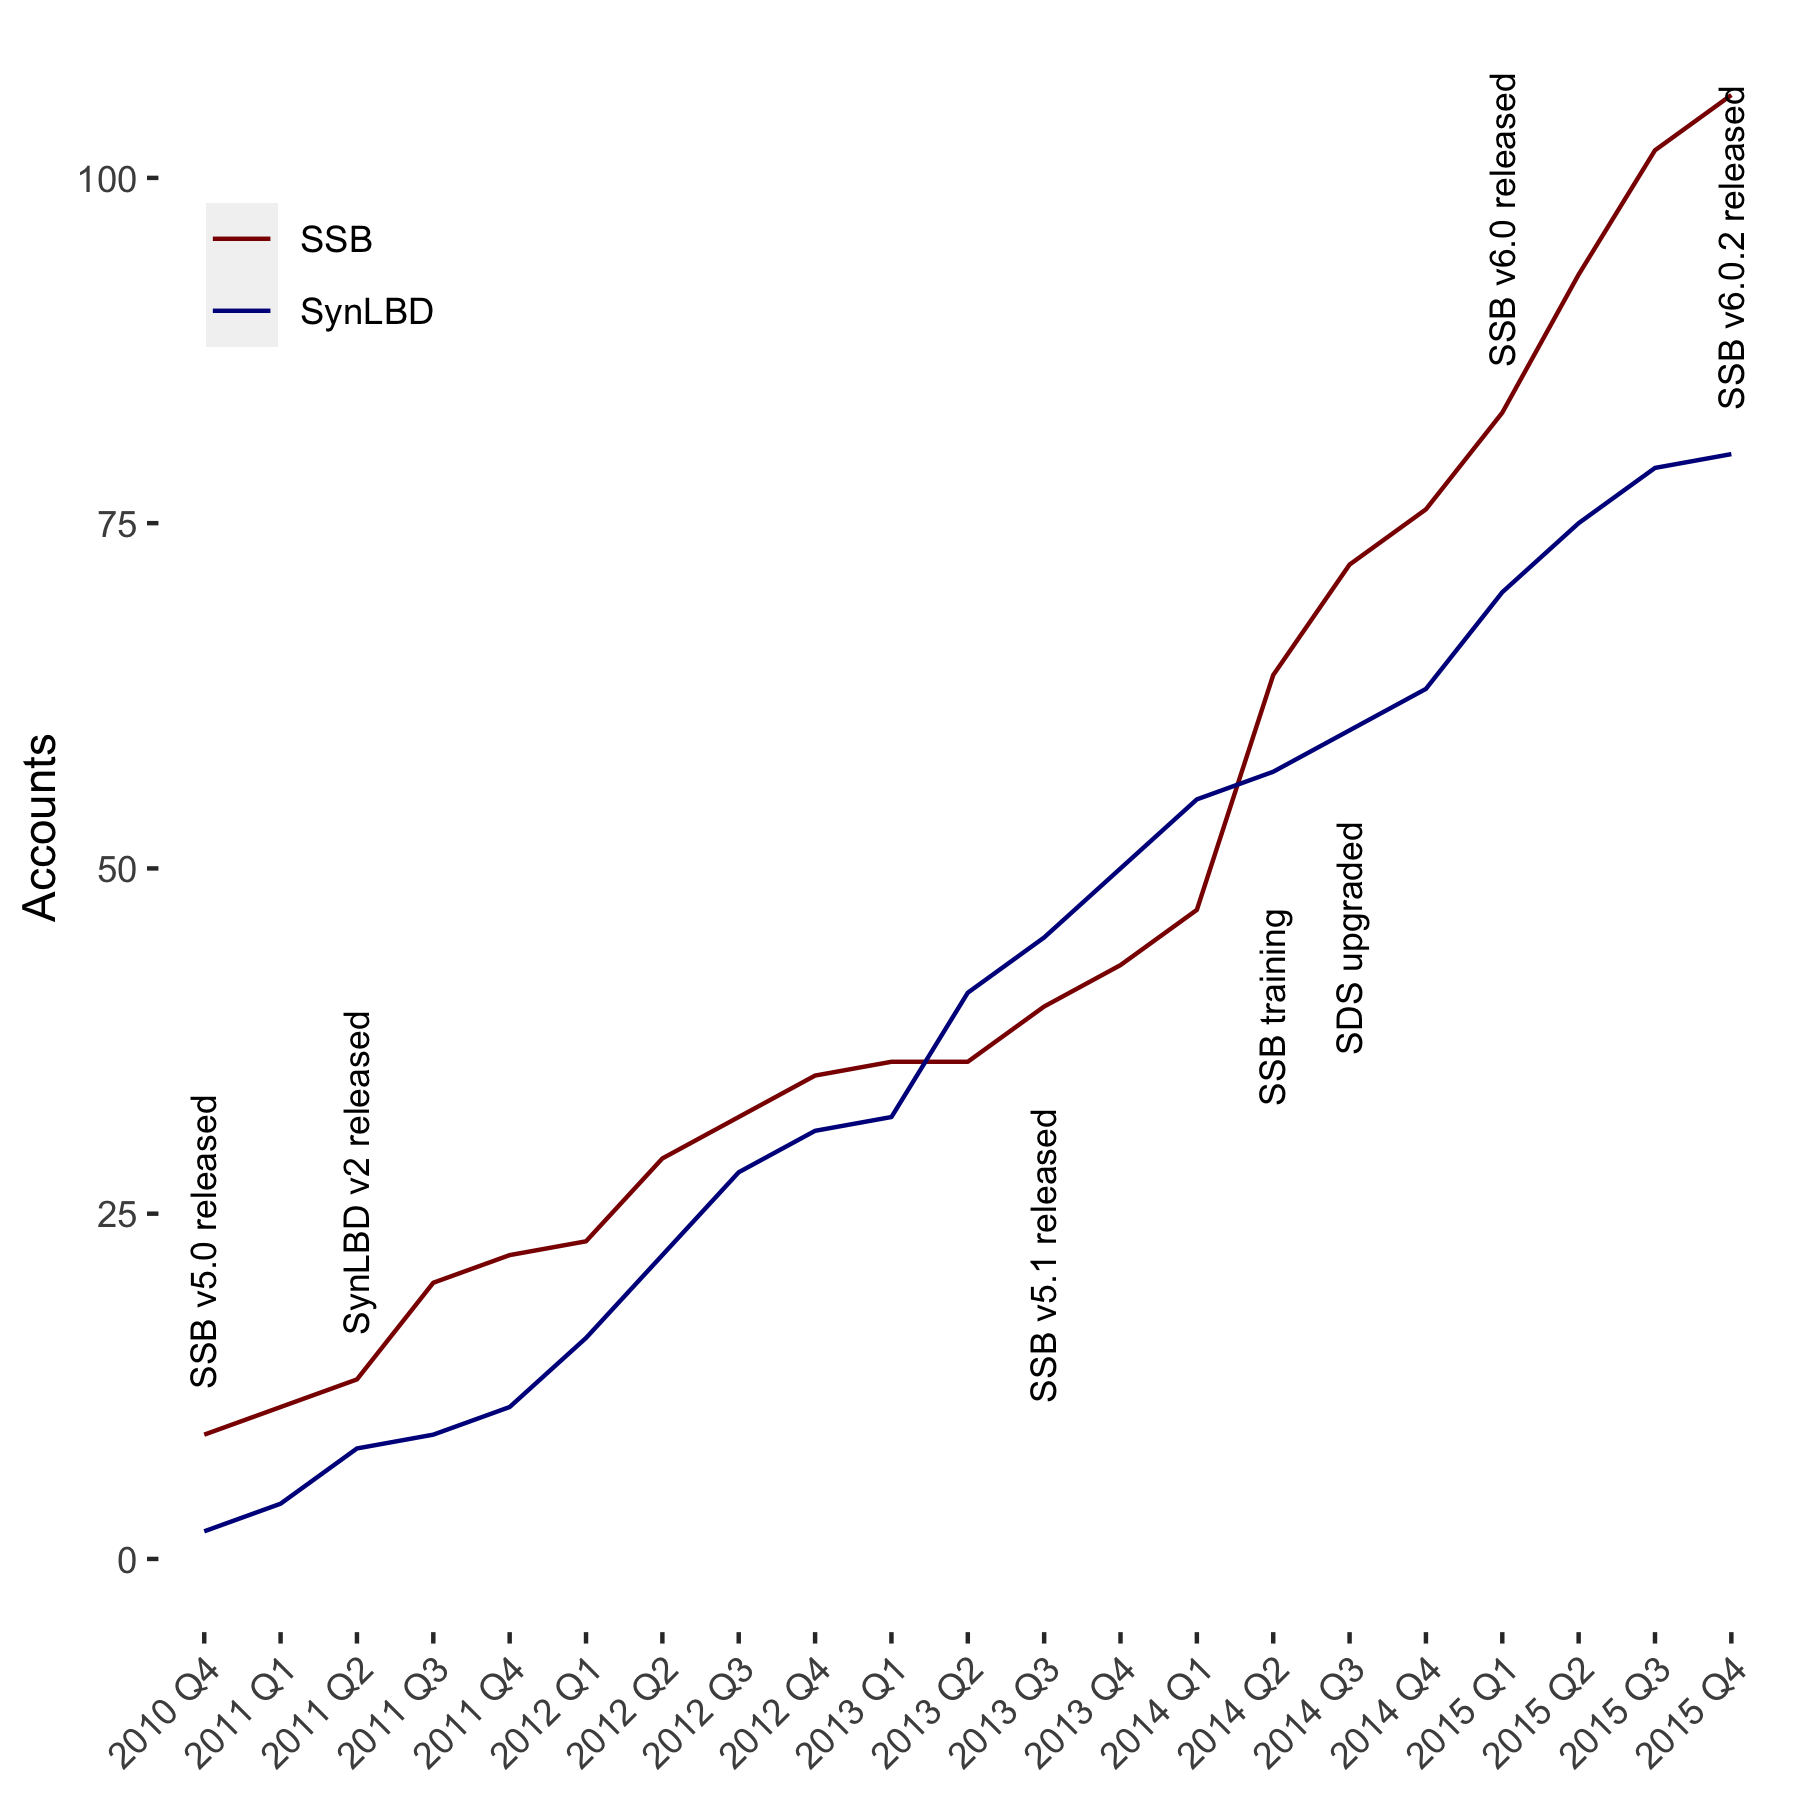
\includegraphics[width=0.7\textwidth]{figs/accounts-2015.png}
    \caption{Computer accounts on the SDS over time}
    \label{fig:growth_in_sds}
\end{figure}

The development cycle was primarily active for the \ac{SSB}. Launched with version 4.1 on the \ac{SDS} in 2010, updates were released in 2013 (v5.1), 2015 (v6.0), and 2018 (v7.0). The version of the \ac{SynLBD} available throughout the time period was v2.0, though additional work to improve the \ac{SynLBD} was undertaken \citep{SJIAOS-2014d}.



%\subsection{Lessons learned from the SDS mechanism}

Several lessons emerged from the SDS mechanism. While many researchers used the data to write papers,
%
and even organized conference sessions specifically around the use of the data,%
%
\footnote{LERA session ``Data Gold! Exploiting the Rich Research Potential of Lifetime
Administrative Earnings Data Linked to the Census Bureau’s
Household SIPP Survey'',  at the Allied Social Sciences 2016 Annual Meeting \citep{american_economic_association_allied_2016}. }
%
even more researchers only ``tried out'' the data. Over 100 researchers were granted access to the server to access the SSB in the first five years of its availability (Figure~\ref{fig:growth_in_sds}), but far fewer published using the SSB data.%
%
\footnote{All publications directly funded by the supporting NSF grant, or using the NSF-funded server, are listed at \url{https://www.zotero.org/groups/5595570/sds-nsf-1042181/library}. Some publications were prepared by NSF-funded project personnel and should not be directly included in a publication count of ``users.'' Most publications were included in this list after a bibliographic full-text search for the grant identifiers. Some researchers may not have reported the published article to the project team, or mentioned the support of the grant to the server they used in their acknowledgements.} 
%
Almost none of the published articles actually used the results produced using the synthetic data. Comparison of parameters obtained from synthetic data and from confidential data using confidence interval overlap, a measure of congruence between the synthetic data and the confidential data introduced by \citet{tas2006}, was very heterogeneous even for a given dataset across and within projects (Table~\ref{tab:overlap}). A more recent assessment, presented as part of this same conference, finds generally similar findings \citep{carr-nber-2023,totty-nber-2023}. Authors were rightly  hesitant to use the parameters estimated on the synthetic data. 


\begin{table}[]
    \centering
    % latex table generated in R 3.4.0 by xtable 1.8-2 package
% Sun Jul 16 15:50:19 2017
\begin{tabular}{llrrrrl}
  \toprule
User & Request & Mean & 75th & 90th & Max & Dataset \\ 
  \midrule
A & 1 & 0.16 & 0.25 & 0.72 & 0.89 & SynLBD \\ 
  A & 2 & 0.10 & 0.00 & 0.52 & 0.92 & SynLBD \\ 
  B & 1 & 0.87 & 1.00 & 1.00 & 1.00 & SynLBD \\ 
  C & 1 & 0.22 & 0.51 & 0.72 & 0.99 & SynLBD \\ 
  D & 1 & 0.49 & 0.79 & 0.87 & 0.98 & SSB \\ 
  E & 1 & 0.39 & 0.56 & 0.63 & 0.94 & SSB \\ 
   \bottomrule
\end{tabular}

    \caption{Distribution of Parameter-specific Confidence Interval Overlap, for selected projects}
    \label{tab:overlap}
\end{table}

Thus, a core goal of the synthetic data --- to replace the confidential data in researchers' analyses --- was not being met, even when the synthetic data actually is a very good test dataset. Nevertheless, the synthetic data were complex enough to allow for development of models without access to the confidential data, what I would call ``good enough data.''

Anecdotal evidence from both my own and Census staff's attempts to use author-provided computer code to run the analysis on the confidential data demonstrated challenges in reproducibility. Authors might hard-code intermediate findings, rather than letting the data drive the analysis, and would otherwise not fully leverage the similarity between the two computing environments. These lead to time-intensive human debugging, or multiple rounds with authors, neither of which are an efficient and satisfying process. 

More interestingly, multiple authors treated the synthetic data access as a gateway process for access to the confidential data. Knowing that the synthetic data did not contain all the features they needed for their analysis, but having to wait for permission to access the more detailed confidential data in the \ac{FSRDC}, authors used the synthetic data to prepare analyses and explore the data. Figure~\ref{fig:useRDC} shows an  analysis of the first 106 users of the SDS, and subsequent usage of the \ac{FSRDC}. 

\begin{figure}
    \centering
    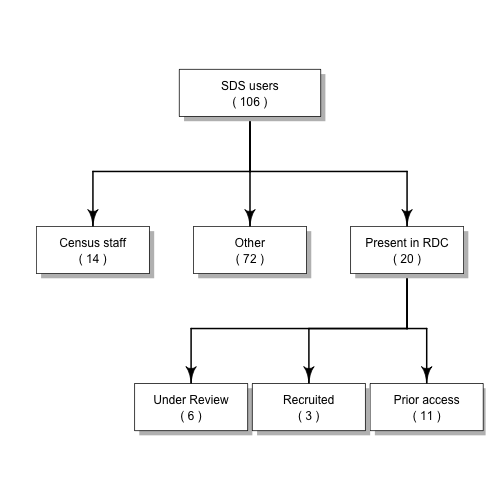
\includegraphics[width=0.5\linewidth]{figs/useRDCgraph.png}
    \caption{SDS users and access to FSRDC}
    \label{fig:useRDC}
\end{figure}

Importantly, in the initial phase of the projects, turnaround (submission of validation request and receipt of validated and privacy-protected results) was quite fast - single-digit weeks, rather than the multi-month process of obtaining access to the \ac{FSRDC}. However, the introduction of new disclosure avoidance procedures at the Census Bureau, and the lack of integration of those procedures into the validation process, greatly increased the time lag in the second half of the projects.

\section{Scaling up access to confidential data via synthetic data}

If data cannot be made available due to intractable disclosure avoidance issues, yet access should be broadened, what can agencies do?  The first-order solution is, of course, to greatly accelerate the process of granting access to the confidential data, but a secondary problem --- reviewing the output  --- may still bind, even if all the security vetting issues are solvable.

The pilot projects described earlier were not set up to scale. Statistical agencies and research institutes have explored various ways to scale up access to confidential data. To cite a few examples, Statistics Canada provides the Real-time Remote Access (RTRA) process, Norway has the Microdata.no system, the Bank of Portugal uses a two-stage system combining a remote desktop and validation \citep{guimaraes_reproducibility_2023}, and \citet{barrientos_providing_2018} proposed a differentially private verification server. 

Many such processes have restrictions that limit their utility for researchers. The aforementioned Statistics Canada and microdata.no systems strongly limit the type of analysis that is feasible by restricting the software keywords that can be used (RTRA), by creating a structured new statistical language (microdata.no), or by limiting the types of analysis that can be run and validated \citep{barrientos_providing_2018}. Users of the Bank of Portugal's system still need to use the remote desktop system, similar to the SDS outlined before, because the data hosted there is not authorized as a full public-use product.

The issue is compounded by well-documented problems with the reproducibility of code in the social sciences. Heuristically, many of the problems with the SDS arose because the code failed to reproduce during validation, even though it was  run in a very similar environment to the development environment. Researchers in the social sciences appear to rely heavily on interactive computing, with code produced subsequently failing simple reproducibility tests. In a sample of over 8,000 replication packages associated with high-profile economics articles, only 30\% had some sort of master script, allowing for ``push-button'' reproducibility.\footnote{Code run in November 2023, searching for any filename that contained the strings `main' or `master', the most common name used for control code in economics.} While ``push-button'' reproducibility may be optional for a general replication package, it is a requirement for a scalable remote-submission system. In part to cater to researchers' demand for interactive systems, remote-access or local secure access in the form of physical or virtual secure data enclaves are still the dominant --- but expensive --- way to access confidential data. The dominant method of access thus forces researchers to choose between lower quality data in an environment that corresponds to their preferred computing method, and higher quality confidential data in environments that are expensive for researchers, data providers, or both.

\subsection{Desiderata}
\label{sec:desiderata}

Drawing on the experience from the SDS pilot projects and other remote access methods used in the past, as well as looking at newer technologies that have emerged in the last decade, I suggest that a new, scalable mechanism to provide access to confidential data should have the following desirable characteristics:

\begin{enumerate}
    \item the mechanism must support arbitrary modeling approaches and ideally a large number of programming languages
    \item the mechanism must allow for development of models by researchers that are close to their ``normal'' method of developing models
    \item the mechanism must be low-cost for the data provider, scaling at best sub-linearly with the number of users of those datasets
    \item the mechanism must be low-cost for the data user, imposing at best marginal costs on their existing research infrastructure (software, computers)
    \item the privacy-protected data provided as part of such mechanisms must be good enough to allow for complex modeling
    \item validation, if necessary, must be fast - on the order of hours
\end{enumerate}

Note that public-use data files, as historically provided by statistical agencies, satisfy all of these criteria, except for the last one, which can take years. Should statistical agencies actually offer validation even for such public use data, as \citet{reiter_verification_2009} have argued? Traditionally, they do not, and leave it up to individual researchers to ``self-validate'' by requesting access to confidential data in a time-consuming fashion.\footnote{See \cite{armour_using_2016} for one example of such a project, affecting the widely-used \ac{CPS}}

\section{A Proposal using Containers}
\label{sec:proposal}

In VILHUBER-HDSR, I demonstrate a simple scenario that satisfies most of the desiderata,  using containers. 
%
The use of containers in this way is novel as a systematic way to provide scalable, potentially high-throughput validation, and differs in usage from previous methods, such as the Cornell Synthetic Data Server. 
%
Containers, often referred to using the name of a particular implementation by a commercial provider (Docker), are technology most often, but not exclusively associated with Linux, which enables computer processes and code libraries to be bundled and constrained.\footnote{In the academic world, Singularity/Apptainer is another container technology typically used in \ac{HPC} environments.} In essence, a container bundles into a single file all the dependencies and code required to run an application or to conduct a researcher's statistical analysis. This file can then be run on any computer without (much) further ado. Containers can be hosted on a cloud platform, but can also run  on researcher compute platforms (laptops).  

Containers are well-understood in the computer science and statistics community \citep{boettiger_introduction_2015,moreau_containers_2023}. However, acceptance in the economics community is not particularly widespread, so far. In the same 8,000 replication packages mentioned earlier, only 0.13\% had used containers. 

The use of containers in the context of synthetic data with validation is to provide users with access to data and coding resources such that their analysis is easily portable, and verifiably reproducible. Within containers, users can implement arbitrary methods of analysis in the statistical programming language of their choice, as most are compatible with containers, even those requiring licenses.%
%
\footnote{For a general example of containers for Stata, see \citet{docker-stata}. For a particularly complex example involving three different licensed software, see \citet{lars_vilhuber_aeadataeditordocker-aer-2023-0700_2024}.}
%
They will need to be aware of constraints imposed by the disclosure avoidance rules \citep{abowd_economic_2015}, just as they would if accessing the confidential data directly, and as they should be if using public-use data. Crucially, containers can  be checked for reproducibility before being forwarded to the confidential computing environment. Once determined to be reproducible, containers can then be extended  to use confidential data, and enable a wide spectrum of plug-in disclosure avoidance measures. Crucially, all checks on reproducibility can be performed prior to validation using the confidential data, on open, possibly commercial platforms. Only once reproducibility is confirmed is the same analysis model ported to the confidential data. 

Containers can be run both locally as well as on cloud infrastructure. The (potential) use of cloud providers removes the requirement for users of the synthetic data to install anything locally, and for statistical agencies to maintain such a public-facing infrastructure. Many academic environments provide some support for running containers, but crucially, academic support is not a requirement, potentially opening up the use of this mechanism to data journalists or citizen scientists. The open-source nature of the container technology allows users to do run containers themselves, when they want to, or when they have to. Thus, a container-based validation mechanism  dramatically reduces the agency's cost of providing access to synthetic data.
%
Containers not only allow for reproducible running of code, but are themselves reproducibly generated. This has favorable IT security implications, since no external software needs to be transferred, a regular problem point for security-conscious agencies. In fact, as I outline in VILHUBER-HDSR, the agency should be the entity defining the container image, exporting it to the public while maintaining a high security posture.

%\subsection{Sending results back to user: output vetting}

Once results have been generated, the usual disclosure avoidance workflow at the data provider is triggered. This might entail post-processing of the results, generation of additional supporting statistics (though these should generally be included in the processing), and finally, provision of the results to users. 
%
Scalability of a system as described here hinges critically on having streamlined output vetting. Ideally, this  part must also be automated. At present, non-automation of output vetting is likely the single most important bottleneck of this system. However, the challenge of creating automated and reliable disclosure avoidance procedures is  not unique to the validation process described here.


\section{Conclusion}

The use of containers ensures reproducibility, reliable portability, and enables scalability. The use of cloud-based commercial services requires no infrastructure or software maintenance by either data provider or users, but is not a necessary condition, as users can easily provide their own infrastructure. Crucially, this means that the cost to statistical agencies of providing users with compute resources is avoided. With very little effort, automation is possible (potentially through web forms), and the only likely constraint to full automation is the absence of automated output vetting algorithms. While containers are not the ``normal'' way of developing statistical models in economics, they are increasingly being used in statistics, and at the cutting edge of the social sciences. 

Thus, containers satisfy most of the desiderata outlined earlier. They do need to rely on synthetic data with sufficient complexity, if not analytical validity, in order to allow for the interactive development of analyses, and a privacy-protection mechanism that can scale. If such a privacy-protection mechanism can be tuned to acceptable protection levels (on par with traditional mechanisms that are applied to unrestricted public-use products), then validation can be made highly automated, and the quality of the synthetic data itself can be decreased, while maintaining high levels of user acceptance due to a fast validation process.

Containers offer the promise of streamlining and improving indirect access to confidential data. As a currently under-utilized technology in the space of the federal statistical agencies, it may be a way to modernize and adapt the way that synthetic data and remote processing interact in a researcher-friendly way.























\section*{Disclosure Statement}
The author have no conflicts of interest to declare. The mention of commercial entities is not meant to endorse any such providers, and the author holds no financial interest in any of the mentioned commercial entities.

\section*{Acknowledgments}

I have benefited from discussions with many folks, including Gary Benedetto, John Abowd, Rob Sienkiewicz, and from feedback following presentations to the National Academies, Census Bureau, and at the NBER conference on ``Data Privacy Protection and the Conduct of Applied Research.'' The original development of the idea was partially funded by \href{https://sloan.org/grant-detail/6845}{Alfred P. Sloan Foundation Grant G-2015-13903}. The Synthetic Data Server project received funding from \href{https://www.nsf.gov/awardsearch/showAward?AWD_ID=1042181}{NSF grant SES-1042181}, \href{https://www.nsf.gov/awardsearch/showAward?AWD_ID=0941226}{NSF Grant BCS-0941226} and from the Alfred P. Sloan Foundation as well as the  Edmund Ezra Day chair at Cornell University.

\section*{Contributions}

LV conceived the topic, wrote the text, and prepared the examples.





% All references should be stored in the file "references.bib"
% Please do not modify anything below this line.
\bibliographystyle{econ}
\bibliography{references,wsc2015,wsc2013,incomplete}


\end{document}
